\documentclass[11pt]{article}
\usepackage[margin=1in]{geometry}
\usepackage{amsmath,amssymb,graphicx,booktabs}
\title{Core-like satellites in a three-site Hubbard chain with positive $U$ (FCI)}
\author{}\date{\today}
\begin{document}\maketitle

\noindent \textbf{Model.} Three sites $c,o,v$ (core, occupied, virtual), four electrons, on-site energies $\epsilon_i$, hoppings $t_{co},t_{ov},t_{cv}$ and only the on-site interaction $U_i\ge0$:
\begin{equation}
H=\sum_{i,\sigma}\epsilon_i n_{i\sigma}+\sum_{i\ne j,\sigma}t_{ij}\,c^\dagger_{i\sigma}c_{j\sigma}+\sum_i U_i\,n_{i\uparrow}n_{i\downarrow}.
\end{equation}
The ground state ($N=4$) should be $\simeq c^2o^2v^0$. The removal spectrum is the exact (FCI) Lehmann sum over the $N=3$ eigenstates $m$: a line at $\mathrm{IP}_m=E^{N-1}_m-E^N_0$ with weight $|\langle m|c_{i\sigma}|0\rangle|^2$ on site $i$ (\texttt{scripts/fci\_trimer.py}; Fock space of 64 states). Weights below are per spin and normalized to 1 for the $c$ orbital. The \emph{main line} is the strongest $c$ line; a \emph{satellite} is $c$ weight at binding energy more than $1$ above it. A point is accepted as a core only if $n_c>1.9$, $n_v<0.3$--$0.4$, the $c$ lines carry less than $10\%$ weight on $o,v$, all weighted IPs are positive, and the $c$ line lies at least $3$ above the $o$ line.

\noindent \textbf{Grid scan.} 23\,040 points ($\epsilon_c\in\{-14,-8\}$, $\epsilon_o=-1$, $\epsilon_v\in\{0.5,2,4\}$, $t_{co}\in[0.3,2.5]$, $t_{ov}\in\{0.5,1,2\}$, $t_{cv}\in[0,2]$, $U_i\in\{0,3,4,6,8\}$ only non-negative). With a deep core ($\epsilon_c+U_c<-3$) the best point is $\epsilon=(-8,-1,0.5)$, $t=(0.6,0.5,1)$, $U=(4,0,6)$: main line $0.939$ at $\mathrm{IP}=4.37$, one satellite of weight $0.0075$ at $\mathrm{IP}=13.4$. Satellites stay below $1\%$.

\noindent \textbf{Optimization.} Differential evolution (6 seeds) maximizing the satellite weight, $U_i\in[0,10]$, $t_{co},t_{cv}\le0.5$, $t_{ov}\le4$, $\epsilon_c\in[-20,-3]$, $\epsilon_o\in[-5,0]$, $\epsilon_v\in[0,8]$, with the core criteria above. Five seeds give the same optimum, satellite weight $0.028$ (the sixth, $0.017$):
\begin{center}\begin{tabular}{ccc|ccc|ccc}\toprule
$\epsilon_c$&$\epsilon_o$&$\epsilon_v$&$t_{co}$&$t_{ov}$&$t_{cv}$&$U_c$&$U_o$&$U_v$\\\midrule
$-13.2$&$-3.55$&$0$&$0.50$&$0.15$&$0.50$&$9.95$&$3.13$&$0.05$\\\bottomrule\end{tabular}\end{center}
with $n=(1.94,1.77,0.29)$. Its removal spectrum is in Fig.~\ref{fig:s}: the $c$ weight is $0.392$ and $0.541$ at $\mathrm{IP}=3.39$ and $3.52$ (a split main line), $0.010$ at $4.77$ and $0.017$ at $16.8$; the $o$ line (weight $0.78$ on $o$, $0.13$ on $v$) is at $0.50$. The upper parameters sit at the bounds ($t_{co},t_{cv}=0.5$, $U_c\approx10$), so the maximum is set by the bounds, and the large $U_c$ makes the $c$ structure Hubbard-like rather than a shake-up.

\begin{figure}[h]\centering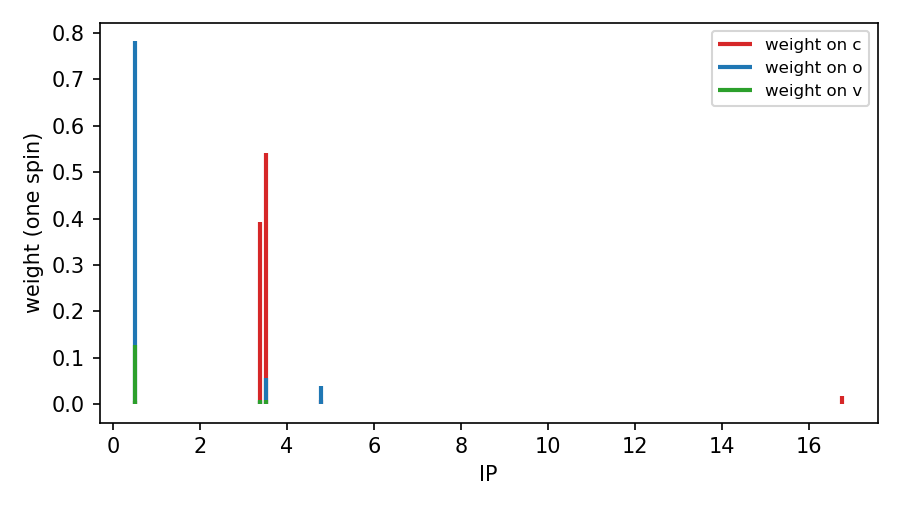
\includegraphics[width=0.6\textwidth]{hubbard_sat_spectrum.png}
\caption{Removal spectrum (one spin) of the best $U\ge0$ point, weights on $c$, $o$, $v$.}\label{fig:s}\end{figure}

\noindent \textbf{Larger hopping.} Letting $t_{co},t_{cv}$ go up to $3$ raises the weight of the second $c$ line to $0.24$ ($\epsilon=(-10.2,-3.95,4.85)$, $t=(2.15,1.91,2.94)$, $U=(0.42,4.56,9.87)$; main line $0.73$ at $\mathrm{IP}=10.82$, second line $0.22$ at $10.02$). This line lies $0.8$ \emph{below} the main line and the parameters are at the bounds with strong $c$--$o$--$v$ hybridization, so it is a level splitting, not a shake-up satellite.

\noindent \textbf{Conclusion.} With on-site $U_i\ge0$, hoppings and local energies only, a core hole reaches $o$ and $v$ only through hopping, so the satellites are weak.
\begin{itemize}
\item \emph{Largest satellite weight with a genuine core (shake-up side):} $0.028$ of the $c$ weight, at $\epsilon=(-13.2,-3.55,0)$, $t_{co}=0.50$, $t_{ov}=0.15$, $t_{cv}=0.50$, $U=(9.95,3.13,0.05)$. Its nature: $0.017$ is a far satellite at $\mathrm{IP}=16.8$ (about $13$ above the main line, a true shake-up-like line) and $0.010$ is a $c$--$o$ mixed line at $4.77$ ($1.3$ above the main line; this line has $0.039$ weight on $o$). The main line itself is split ($0.39+0.54$ at $3.39$, $3.52$; two lines $0.13$ apart), with $U_c\approx10$ and $t_{co},t_{cv}=0.5$ at the optimizer bounds.
\item \emph{Largest weight overall:} $0.24$, at $\epsilon=(-10.2,-3.95,4.85)$, $t=(2.15,1.91,2.94)$, $U=(0.42,4.56,9.87)$. Its nature: a level splitting of $c$ by strong $c$--$o$--$v$ hybridization (second line $0.8$ below the main line), not a shake-up.
\item \emph{Cleanest deep core (grid):} $\epsilon=(-8,-1,0.5)$, $t=(0.6,0.5,1)$, $U=(4,0,6)$: qp $0.939$, satellite $0.0075$ at $\mathrm{IP}=13.4$.
\end{itemize}
\end{document}
